% !TEX root = ../../presentation.tex

\begin{slide}{Kernel Layer}
  \pause
  \begin{tikzpicture}
    \begin{axis}[samples=64, domain=-7:+7]
      \addplot[mark=none]{1/(1+exp(-x))};
  \end{axis}
  \end{tikzpicture}

  \textbf{Sigmoid Activation Function}
\end{slide}

\begin{slide}{Kernel Layer}
\begin{columns}
  \begin{column}{0.5\textwidth}
    \centering
    \pause
    {\large$\sigma(z) = \frac{1}{1 + e^{-z}}$}

    \vspace{0.5cm}
    \href{https://eigen.tuxfamily.org/dox/unsupported/TensorFunctors_8h_source.html}{\textbf{Forward Pass}}
  \end{column}
  \begin{column}{0.5\textwidth}
    \pause
    {\large$\sigma'(z) = \sigma(z)(1 - \sigma(z))$}

    \vspace{0.48cm}
    \hspace{0.4cm}\href{https://github.com/tensorflow/tensorflow/blob/2c8d0dca978a246f54c506aae4587dbce5d3bcf0/tensorflow/core/kernels/cwise_ops_gradients.h\#L51}{\textbf{Backward Pass}}
  \end{column}
\end{columns}
\end{slide}

\begin{slide}{Quantization}
  \begin{tikzpicture}[thick]
    \tikzset{op/.style={draw, rectangle, text width=0.8cm,%
                        text height=0.4cm, rounded corners=1pt}};
    \tikzset{var/.style={draw, circle, inner sep=8pt}};

    \path (-4, 0) coordinate [var] (z) node {$z$};
    \path (0, 0) coordinate [var] (s) node {$\sigma$};

    % Quantize Node
    \onslide<2-> {
      \path (2, 0) coordinate [op] (Q) node {\tiny\textbf{Quantize}};
      \draw [->] (s) -- (Q);
    }

    % Edges
    \draw [->] (z) -- (s);
    \onslide<1>{
      \draw [dotted, ->] (s) -- (4, 0);
    }
    \onslide<2->{
      \draw [dotted, ->] (Q) -- (4, 0);
    }

    % Scale
    \only<3-> {
      \foreach \t/\f/\q in {-2/0/0,%
                            -1/0.25/64,%
                            0/0.5/128,%
                            +1/0.75/192,%
                            +2/1/256} {
        \ifnum\q<192
          \draw [|-] (\t, -2) -- +(1, 0);
        \else
          \ifnum\q=192
            \draw [|-|] (\t, -2) -- +(1, 0);
          \fi
        \fi
        \draw (\t, -2.5) node {\tiny$\f$};
        \draw (\t, -1.5) node {\tiny$\q$};
      }
    }

  \only<4-> {
    \draw (0, -3.8) node {\footnotesize\texttt{github.com/google/gemmlowp}};
  }
  \end{tikzpicture}
\end{slide}
